
\chapter{Host parasite interactions} % Chapter title

\label{ch:01-01} % For referencing the chapter elsewhere, use \autoref{ch:name} 


A large number of organisms throughout the tree of life establish stable interactions with different species. These interactions are often classified according to their perceived impact on the fitness of their members. We traditionally talk about parasitism for interactions with one-way benefits, and mutualism when the interaction has a positive impact on all parties involved. Rather than a dichotomous classification, the difference between parasitism and mutualism is better viewed as a spectrum, depending on the \Gls{fitness} cost and benefit of the relationship to the host (Fig. \ref{fig:01-01:mutualism}).

\begin{figure}[b]
    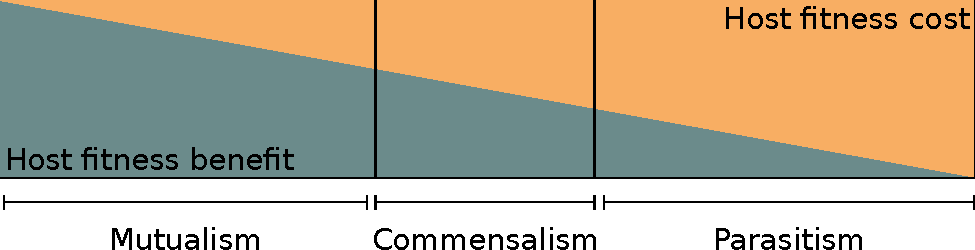
\includegraphics[width=\textwidth]{Parts/Part01/gfx/parasitism_mutualism.pdf}
    \caption{Parasitism - Mutualism spectrum: A spectrum of host \Gls{fitness} cost underlies common terms used to described a biological interactions.}
	\label{fig:01-01:mutualism}
\end{figure}

Biological interactions are observed at different scales, from nanometer-scale virophages infecting giant viruses to fungi forming mycorrhyzal networks spanning several meters \citep{johnsonFunctioningMycorrhizalAssociations1997,selosseMycorrhizalNetworksLiaisons2006} allowing exchange of nutrients with plants root systems. These interactions shape the evolutionary trajectories of the species involved and their genomic landscapes. These changes can sometimes result in drastic transitions in the organisms' lifestyle. 

This can be the case for example with intracellular bacteria forming symbiosis with their host cells, known as endosymbionts. The \textit{Wolbachia} genus is a famous example of endosymbiotic bacteria infecting arthropod species. These bacteria are reproductive parasites which can be transmitted vertically through infection of the host female's eggs \cite{knightMeetHerodBug2001}. Some \textit{Wolbachia} have altered the reproductive capabilities of their sexual host species to reproduce asexually by \Gls{parthenogenesis} \cite{stouthamerMolecularIdentificationMicroorganisms1993}. This effectively removes all males from the host population, benefitting the bacterium which can only be transmitted through females. In some species, infection by \textit{Wolbachia} has even become necessary for reproduction. While the bacterium takes advantage of its host reproduction, it also provides numerous advantages such as resistance to viruses in flies and mosquitoes \citep{hedgesWolbachiaVirusProtection2008,teixeiraBacterialSymbiontWolbachia2008} and help with vitamin synthesis in bed bugs \cite{nikohEvolutionaryOriginInsectWolbachia2014}, illustrating the blurry line between parasitism and mutualism.

In this work, we focus on bacterial endosymbionts. Living directly inside of their host's cytoplasm, their genomic fate is most tightly linked to their host.

\section{The evolutionary context of intracellular parasitism}

Intracellular bacteria can either be facultative or obligatory endosymbionts. Obligatory endosymbionts can only replicate inside of their host cells. This is the case of several genera of obligate intracellular bacteria, such as \textit{Rickettsia} or \textit{Chlamydia}. These parasites are unable to reproduce outside of their host and become reliant on it for most metabolic pathways. The host cytoplasm being an isolated environment, obligate intracellulars have limited opportunity for recombination with other strains. Small populations of asexual organisms unable to recombine are at the mercy of \Gls{Muller}, the progressive accumulation of mutations and loss of genetic material. They undergo a process known as genome reduction: Pathways provided by the host need no longer be encoded by the parasite and are therefore lost \cite{mccutcheonExtremeGenomeReduction2012}. This process eventually leads to the parasite becoming completely reliant on its host for survival.

Facultative parasites bacteria opt for a different strategy, often with larger host ranges. These bacteria can complete their life cycle without the need for a host. They can reproduce in the extracellular space and be transmitted between different species. An analogy often used to describe the evolutionary dynamics of intracellular parasites with their hosts is the "arms race". Each organism evolves novel strategies (i.e. weapons) to improve its own fitness at the expense of the other. This is the case for intracellular bacteria such as \textit{Legionella} or \textit{Salmonella}, which can secrete a large arsenal of effector proteins into their host's cytoplasm. These proteins will manipulate host pathways to sustain the parasite's reproduction and protect it against host defenses. Many of these proteins are redundant in the sense that they interact with the same host proteins or pathways and can complement each other if one is defective \cite{ghoshParalogsMultipleLayers2017}.

Perfectly redundant genes should be subject low selective pressures, making them susceptible to genetic drift and therefore unstable \cite{bergthorssonOhnoDilemmaEvolution2007}. It is therefore thought that the functions of redundant genes in intracellular bacteria have partial overlap, such as different affinity for certain substrates or the ability to function in different conditions or infection stages \cite{ghoshParalogsMultipleLayers2017}. Selective pressure would therefore be applied on these specificities. This is likely an important phenomenon for parasites with a broad host range or environments susceptible to changes.

Most intracellular bacteria incorporate genes from their hosts into their genome. Such genetic transfers are known as \acrfull{HGT} and are a major contributor to bacterial genomes, with an estimated 80\% of genes being ionvolved in HGT at some point in their history \cite{daganModularNetworksCumulative2008}. More recently, HGT from bacteria to eukaryotes have also been detected in eukaryotic genomes. Although they are much less frequent 0.04-6.49\% of genes in microbial eukaryotes \cite{vanettenHorizontalGeneTransfer2020}), gene transfers from intracellular microorganisms to eukaryotic hosts are thought to have catalyzed major shifts in environmental niche. Examples are the terrestrial colonization of plants and extremophile eukaryotes such as sea ice diatoms which acquired ice binding proteins from prokaryotes \cite{vanettenHorizontalGeneTransfer2020}.

All these exchanges illustrate the complex evolutionary dynamics of intracellular life; genetic material can be passed not only from the host to the parasite, but also between different endosymbionts and to the host.

\section{Amoeba as a host model}

Free living amoeba are ubiquitous unicellular organisms found in soil and various bodies of water, such as rivers, lakes \cite{johnSeasonalDistributionPathogenic1995} or even puddles \cite{sakamotoLegionellaPneumophilaRainwater2009}. They graze on bacterial biofilms, feeding on microorganisms by phagocytosis. This lifestyle exposes them to a large number of bacteria and viruses and they are host to many endosymbionts. 

Amoeba offer a great experimental model, as many species are easy to grow in laboratory conditions and can be used for infection experiments. Despite their extensive use as an infection model, only a few species have high quality genome assemblies available, and the genomics of free living amoeba are still largely unknown. For example the \textit{Acanthamoeba castellanii} genome has evidence for highly variable ploidy levels \cite{maciverAsexualAmoebaeEscape2016} and horizontally acquired genes \cite{clarkeGenomeAcanthamoebaCastellanii2013}. These peculiar genomic features are likely important in their interactions with endosymbionts. Indeed, high ploidy levels have been proposed as a mean for asexual amoeba to escape \Gls{Muller} through homologous recombination between haplotypes \cite{maciverAsexualAmoebaeEscape2016}.

% HGT to counter muller's ratchet (Nowack2016)
Similarly, the amoeba \textit{Paulinella chromatophora} has photosynthetic organelles whose genome benefits from HGT from endosymbionts, as they counteract \Gls{Muller}. This interesting observation, provides an interesting track to explain the conservation of horizontal gene transfers in the genome of free living amoeba \textit{A. castellanii} \cite{clarkeGenomeAcanthamoebaCastellanii2013}.

Their long term coevolution with endosymbionts make free living amoeba an interesting model for evolutionary biology and ecology, but they are also an important organism for public health as they are the reservoir of human pathogens such as \textit{Legionella pneumophila}. Besides, many free living amoeba have a biphasic life cycle, living as trophozoite to feed and reproduce, and transforming into cysts in harsher conditions. This encystation process makes them even more important from the standpoint of public health; intracellular bacteria infecting amoeba are able to survive water chlorination or antibiotic treatments by using the encysted amoebae as shelters.

\section{\textit{Legionella pneumophila}}

\textit{L. pneumophila} is an important model for studying intracellular bacteria and infects a range of 15 species of amoebae and ciliated protozoa in the wild \cite{rowbothamPreliminaryReportPathogenicity1980}. It can also infect lung macrophages of humans and other mammalians. In humans, this can cause a severe pneumonia known as \textit{Legionnaire's disease} \cite{edelsteinLegionnairesDiseasePontiac2014}. Human to human transmission of \textit{L. pneumophila} is extremely rare \cite{correiaProbablePersontoPersonTransmission2016}, making infection of macrophages an evolutionary dead-end for the bacterium. \textit{L. pneumophila} is a major public health concern as it can contaminate water distribution systems and cause major outbreaks. The outbreak which lead to the identification of this bacterium and after which the bacteria was named happened at a convention of the American legion, Philadelphia, in 1976. This outbreak resulted in 182 cases, 29 of whom died. Since then, outbreaks are associated to \textit{Legionella} every year with over 32,000 cases reported between 1995 and 2005 \cite{mcdadeLegionellaPreventionLegionellosis2008}.

Unlike other bacteria on which phagocytic cells prey (Fig. \ref{fig:01-01:legionella}a), when it is engulfed by a predatory cell, \textit{Legionella} evades the lysosomal degradation route and survives in a special vacuole, the \acrfull{LCV} (Fig. \ref{fig:01-01:legionella}b). It does so using its type IV secretion system to secrete around 300 effector proteins into the host cytoplasm and rewire the host metabolic and signalling pathways. Many of those effectors contain eukaryotic domains and likely originate from inter-domain \acrshort{HGT} \cite{felipeEvidenceAcquisitionLegionella2005}. Through their secretion, the bacterium is able to create a niche inside of the host cell with stable conditions and ample nutrients nutrients where it can proliferate.


\begin{figure}[b]
    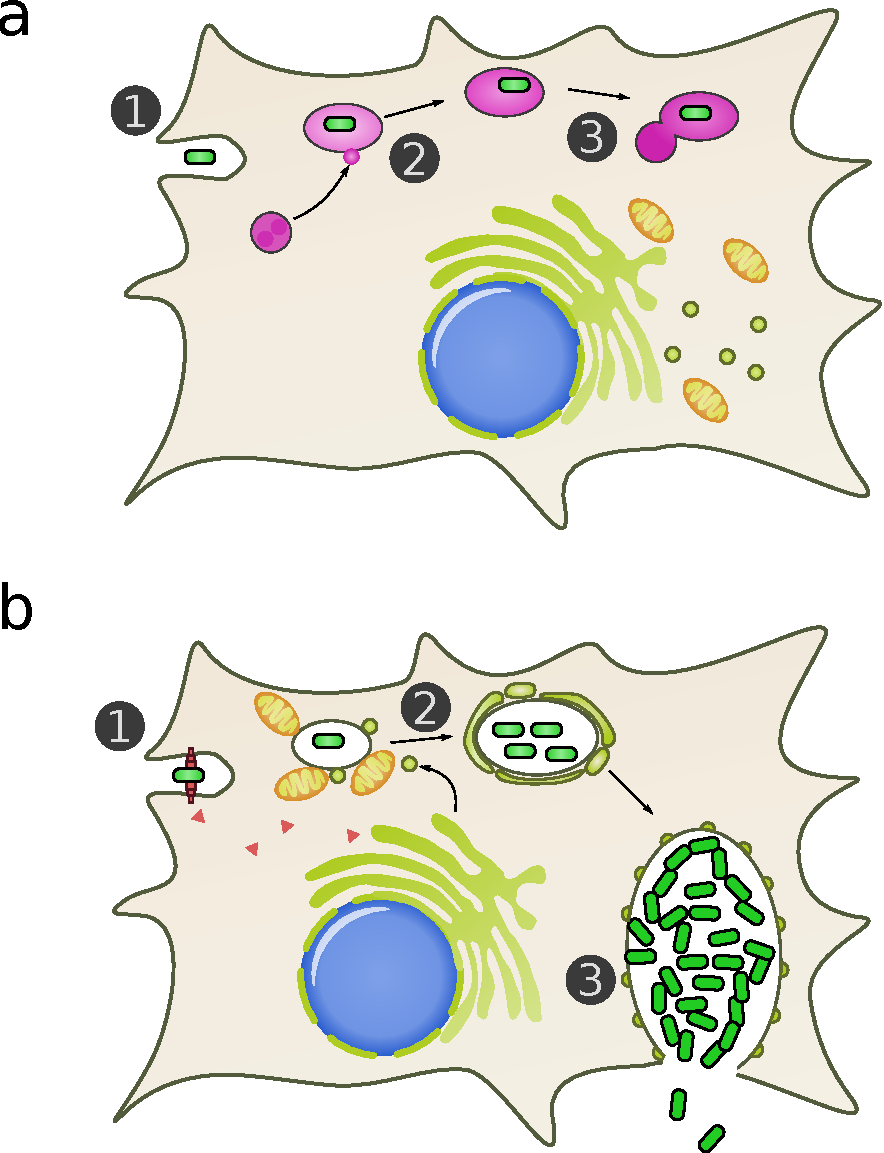
\includegraphics[width=\textwidth]{Parts/Part01/gfx/legionella_life_cycle.pdf}
    \caption{Infection by \textit{Legionella}: \textbf{a}: Non infectious bacteria (green) are phagocytized by amoeba or macrophages (1), the early and late endosomes (pink) acidify the compartment (2), and it finally merges with the lysozome (3) where the bacteria is degraded. \textbf{b} Upon phagocytosis, \textit{Legionella} uses its type IV secretion system to secrete effector proteins (red triangles) into the cytoplasm and evades the endosome route (1). Instead, it stays in a "\textit{Legionella} containing vesicle" (LCV) and recruits mitochondria (orange) and endoplasmic reticulum-derived vescicles (yellow) (2). The bacteria keeps replicating in the LCV until it bursts out and infects other cells.}
	\label{fig:01-01:legionella}
\end{figure}

\subsection{Life cycle}
\textit{L. pneumophila} follows a biphasic life cycle. It can survive in the extracellular environment and thrives in fresh water. It can eith spread planktonically as a free living organism using its flagella to reach new hosts, or by associating with biofilms \citep{hilbiLegionellaSppOutdoors2011,steinertLegionellaPneumophilaAquatic2002}. This extracellular phase is called the "transmissive form", as bacteria will search for new host cells but will not replicate \cite{byrneExpressionLegionellaPneumophilaVirulence1998}. In contrast, when entering a host cell, the bacterium enters the "replicative form". In that phase, the  bacterium takes advantage of the abundant resources and nutrient available in the host cell to replicate as much as possible.

Switching between replicative and transmissive phases requires consequent morphogenetic and metabolic changes, mobilizing expression changes in almost half of the known genes \cite{steinertLegionellaPneumophilaAquatic2002}. Low nutrient and high stress conditions, cause \textit{L. pneumophila} to enter transmissive phase, activating genes related to motility and virulence, such as its type IV secretion system. When entering the replicative phase, genes related to sugar and gluconate uptake and amino-acid catabolism are upregulated instead. The bacteria become acid resistant and replicate in the \acrshort{LCV} until the nutrient pool is depleted.

Comparison of gene expression profiles between \textit{L. pneumophila} grown \textit{in vitro} in the absence of host, and \textit{in vivo} with the amoeba \textit{A. castellanii} revealed that changes associated with progression from exponential growth to stationary phase are similar to those observed between replicative and transmissive phases \cite{bruggemannVirulenceStrategiesInfecting2006}. In \textit{in vitro} cultures, stationary phase refers to the time when bacteria stop replicating for lack of nutrients. This suggests that the biphasic life cycle of \textit{L. pneumophila} is governed by the presence of nutrient in the environment \cite{olivaLifeCyclePneumophila2018}.

The master regulator underlying this switch is thought to be the Carbon storage regulator protein A (CsrA). CsrA is an RNA binding protein with over 400 target transcripts identified, including 40 effector proteins and genes related to virulence and motility. In replicative phase, CsrA binds its target transcripts to repress their translation. When nutrients are running low, \textit{L. pneumophila} produces the alarmone (p)ppGpp, which triggers the expression of noncoding transcripts with strong affinity for CsrA. This prevents CsrA from binding its targets and enables the translation of virulence genes \cite{sahrLegionellaPneumophilaGenome2017}.

\subsection{Host interactions}

While inside the host, \textit{L. pneumophila} consumes products from the host cell for energy production. It relies mainly on serine, threonine and other amino acids but can also scavenge carbohydrates such as gluconate \cite{bruggemannVirulenceStrategiesInfecting2006}. Those nutrients are transferred from the host cytoplasm to the LCV by transporters on the LCV membrane \cite{wielandIntracellularMultiplicationLegionella2005}. The bacterium can increase the availability of nutrients in the host cell using its effector proteins. One example is the AnkB effector which can poly-ubiquitinate host proteins, causing their degradation by the host proteasome, resulting in amino acids which can then be imported into the LCV and consumed \cite{priceMolecularMimicryFBox2009}.
Other effectors block host protein translation to increase the pool of free amino acid available for consumption by \textit{L. pneumophila} \cite{leonPositiveNegativeRegulation2017}.

The host trafficking system is hijacked to recruit mitochondria and \acrfull{ER} membrane vesicles to the LCV. This is likely achieved by modulating the activity of host GTPases, such as Arf1, Sar1 and Rab1 \cite{isbergLegionellaPneumophilaReplication2009}. Some \textit{Legionella} effectors directly affect the host actin cytoskeleton, which is important in many cellular processes including vesicle trafficking \citep{liuLegionellaEffectorDisrupts2017,francoLegionellaPneumophilaEffector2012}.

\textit{L. pneumophila} also ensures successful infection by promoting host cell survival. The effector SdhA interferes with host cell apoptosis by inhibiting caspases \cite{lagunaLegionellaPneumophilatranslocatedSubstrate2006}. All these interferences with host cell signalling pathways are likely bound to affect its expression programm but it was recently found that one of the effectors secreted by \textit{L. pneumophila} directly affects the host epigenetic state. This effector, named RomA, is a histone methyltransferase which can alter the histone methylation state throughout the host genome and affects the expression of a large number of genes \cite{rolandoLegionellaPneumophilaEffector2013}.

There is still much to learn about the interaction between \textit{Legionella} effectors and its host regulation, but direct modification of nucleosomes reveals a new level of intimacy between bacterial endocymbions and their host. Besides, epigenetics and gene expression are tightly connected with spatial genome organization in eukaryotes. This gives a new promising angle to approach the study of host-pathogen interactions.

\section{\textit{Salmonella enterica}}

Unlike \textit{L. pneumophila}, \textit{S. enterica} species are known to infects various birds, reptiles and mammals \cite{uzzauHostAdaptedSerotypes2000}. It is also a model for intracellular bacterial infections and a major human pathogen. \textit{Salmonella} is a facultative intracellular parasite which can infect macrophages, dendritic and epithelial and microfold (M) cells. It is usually transmitted by ingestion of contaminated food and colonizes the gastrointestinal tract. \textit{Salmonella} isolates are classified into 2,500 serovars based on their lipopolysaccharides and flagellar antigens. While most serovars, referred to as "non-typhoidal" cause salmonellosis, a self-limiting enteritis, "typhoidal" serovars are human restricted and cause a systemic disease known as typhoid fever \cite{larockSalmonellaeInteractionsHost2015}.

Every year, it is estimated that there are 16.6 million cases of typhoid fever causing 600,000 deaths in the world, and 1.3 billion cases of acute gastroenteritis associated with \textit{Salmonella}, responsible for 3 million deaths \cite{pangTyphoidFeverOther1995}. Most of the current knowledge on \textit{Salmonella} infection biology was built on the non-typhoidal serovar \textit{S. enterica} subsp. \textit{enterica} serovar Typhimurium \cite{larockSalmonellaeInteractionsHost2015}. 

Much like \textit{Legionella}, when \textit{Salmonella} enters the host cell, it is engulfed into a \acrfull{SCV}  and secretes effector proteins into the host cytoplasm. This is done via two independent type 3 secretion systems (T3SS) named SPI1 and SPI2. These two systems are encoded by and named after the \textit{Salmonella pathogenicity island}, which \textit{Salmonella} likely acquired through horizontal gene transfer.

The mechanisms employed by \textit{Salmonella} to infect host cells are similar to \textit{Legionella}. For example, they encode effectors that also activate the host gene Arf1 to promote bacterial uptake and actin polymerization \cite{larockSalmonellaeInteractionsHost2015}.
